\RequirePackage{fix-cm}
\documentclass[%
    twoside, openright, titlepage, numbers=noenddot,%
    cleardoublepage=empty,%
    %abstractoff,%
    abstract=false,
    BCOR=5.5mm, paper=a5, fontsize=10pt,% A5 soft cover
    %BCOR=5.5mm, paper=17cm:24cm, fontsize=10pt,% 17 cm x 24 cm
    %BCOR=5mm, paper=15.59cm:23.39cm, fontsize=10pt,% Royal soft cover
    %BCOR=0mm, paper=15.24cm:22.86cm, fontsize=10pt,% US-Trade hard cover
]{scrreprt}
\usepackage{etex}
\reserveinserts{10}

% File encoding
\usepackage[utf8]{inputenc}

% Languages
\usepackage[main=english,ngerman]{babel}

% classicthesis setup
\PassOptionsToPackage{%
  %drafting,%
  %dottedtoc,%
  eulerchapternumbers,
  %listings,%
  %parts,%
  floatperchapter, pdfspacing,%
  beramono,%
  %minionprospacing,
  %subfig,%
  %eulermath,%
  a5paper,%
}{classicthesis}

% Meta
%
% Document information
%

\usepackage{etoolbox}    % for \newcounter + patching if needed

% Work version info

\newcounter{worktodocount}
%\newcommand{\worktodo}[1]{
\DeclareRobustCommand{\worktodo}[1]{%
  \stepcounter{worktodocount}%
  \textcolor{red}{\textbf{TODO}: #1}%
}

\usepackage{scrtime}
\newcommand{\workdraft}{\textcolor{gray}{Draft, \today{}---\thistime}}
% \renewcommand{\workdraft}{}
% \renewcommand{\worktodo}{}

\newcommand{\myTitle}{%
  Variance reduction in lattice determinations of the leading order hadronic vacuum polarisation contribution to the muon g-2\xspace%
}
\newcommand{\myPlainTitle}{%
  Variance reduction in lattice determinations of the leading order hadronic vacuum polarisation contribution to the muon g-2\xspace%
}

\newcommand{\myDissNumber}{31433}
\newcommand{\myName}{Roman Maurice Gruber\xspace}
\newcommand{\myUni}{\protect{ETH Z\"urich}\xspace}
\newcommand{\myLocation}{Z\"urich\xspace}
\newcommand{\myTime}{2025\xspace}

% DOI
\newcommand{\myDOI}{10.3929/ethz-c-000783366} % check https://www.research-collection.ethz.ch/workspaceitems/640421/edit


% Hyphenation

\hyphenation{nano-elec-tro-nic}
\hyphenation{openQxD}
\hyphenation{OpenQxD}
\hyphenation{openQCD}
\hyphenation{OpenQCD}


% Common symbols / abbreviations
\usepackage{xspace}

\newcommand{\ie}{i.\,e.\xspace}
\newcommand{\Ie}{I.\,e.\xspace}
\newcommand{\eg}{e.\,g.\xspace}
\newcommand{\Eg}{E.\,g.\xspace}

\newcommand{\quda}{QUDA\xspace}
\newcommand{\Quda}{QUDA\xspace}
\newcommand{\qudas}{QUDAs\xspace}
\newcommand{\Qudas}{QUDAs\xspace}
\newcommand{\openqxd}{openQxD\xspace}
\newcommand{\openqcd}{openQCD\xspace}
\newcommand{\Openqxd}{OpenQxD\xspace}
\newcommand{\Openqcd}{OpenQCD\xspace}
\newcommand{\bigO}{\mathcal{O}}
\newcommand{\observable}[1]{\mathcal{#1}}
\newcommand{\NULL}{NULL\xspace}
\newcommand{\posix}{posix\xspace}
\newcommand{\Posix}{Posix\xspace}

\newcommand{\txyz}{txyz\xspace}
\newcommand{\xyzt}{xyzt\xspace}

\newcommand{\QED}[1]{QED$_\text{#1}$\xspace}
\newcommand{\QEDC}{\QED{C}}

\newcommand{\lat}[1]{\Lambda_{\text{#1}}}
\newcommand{\RCstar}{RC$^{\star}$\xspace}
\newcommand{\Cstar}{C$^{\star}$\xspace}
\newcommand{\CstarHeading}{C\texorpdfstring{$^{\star}$}{*}\xspace}

\newcommand{\x}{×\xspace}

\newcommand{\ggrp}[2]{#1(#2)}
\newcommand{\liealg}[2]{\mathfrak{#1}(#2)}

\newcommand{\cswsu}[1]{c_{\text{SW}}^{\ggrp{SU}{#1}}}
\newcommand{\cswu}[1]{c_{\text{SW}}^{\ggrp{U}{#1}}}

\newcommand{\Dw}{{D_{\mathrm{w}}}}

\newcommand{\openmp}{openMP\xspace}
\newcommand{\Openmp}{OpenMP\xspace}

\newcommand{\openmpi}{openMPI\xspace}
\newcommand{\Openmpi}{OpenMPI\xspace}

\newcommand*\dd{\mathop{}\!\mathrm{d}}
\newcommand*\DD{\mathop{}\!\mathcal{D}}

\newcommand{\spinhalf}{spin-$\frac{1}{2}$\xspace}
\newcommand{\Nst}{N_{\text{st}}} % number of stochastic sources
\newcommand{\Nc}{N_{\text{c}}} % number of eigenmodes sources
\newcommand{\id}{\mathbb{1}} % identity matrix

\newcommand{\Lt}{L_0} % extent in time
\newcommand{\Lx}{L_1} % extent in x-direction
\newcommand{\Ly}{L_2} % extent in y-direction
\newcommand{\Lz}{L_3} % extent in z-direction

\newcommand{\vect}[1]{\vec{#1}}
%\newcommand{\vect}[1]{\mathbf{#1}}

\newcommand{\exptime}{\left\{ 0, \ldots \Lt-1 \right\}}  % explicit temportal lattice set
\newcommand{\expspin}{\left\{ 0, \ldots N_s-1 \right\}}  % explicit spin index set
\newcommand{\expcolor}{\left\{ 0, \ldots \Nc-1 \right\}} % explicit color index set
\newcommand{\expspace}{\left\{ \vect{x} = (x_1,x_2,x_3) \in \mathbb{N}^3 \; \middle| \; 0 \leq x_i < L_i \right\}}

%\newcommand{\ispin}{\text{spin}} % spin index set
%\newcommand{\icol}{\text{color}} % color index set
%\newcommand{\ilat}{\text{lattice}} % lattice index set
%\newcommand{\ispace}{\text{space}} % spatial lattice index set
\newcommand{\stime}{\{ 0, \ldots \Lt-1 \}} % lattice time set explicit

\newcommand\vslattice{\mathcal{V}}  % lattice vector space

% notation for coarse objects; hat or widehat
\usepackage{xparse} % loads expl3
\ExplSyntaxOn
\NewDocumentCommand{\coarse}{m}{ % coarse operator
    \int_compare:nTF { \tl_count:n { #1 } > 1 }
        { \widehat{#1} }
        { \hat{#1} }
}
\ExplSyntaxOff

\newcommand{\restrictor}{R}       % restrictor
\newcommand{\prolongator}{T}      % prolongator

\newcommand{\tslice}[1]{\langle {#1} \rangle} % time slice notation for stochastic estimator

\newcommand{\lattice}{\mathbb{L}}       % represents the lattice
\newcommand{\idxset}{\mathcal{I}}       % all lattice indices
\newcommand{\idxspace}{\Sigma}          % spatial lattice set
\newcommand{\idxtime}{\mathcal{T}}      % temporal lattice set
\newcommand{\idxspacetime}{\Lambda}     % spacetime lattice set
\newcommand{\idxspin}{\Xi}              % spin index set
\newcommand{\idxcolor}{\mathfrak{C}}    % color index set
\newcommand{\idxchiral}{\mathfrak{X}}   % chirality index set

\newcommand{\cexpcolor}{\left\{ 0, \ldots \coarse{\Nc}-1 \right\}}

% spinor product, scalar product
\newcommand{\sprod}[2]{\left({#1}, {#2}\right)} % (A, B)
%\newcommand{\sprod}[2]{\langle #1, #2 \rangle)} % <A, B>
%\usepackage{braket}
%\newcommand{\sprod}[2]{\braket{#1}{#2}} % <A | B>

\newcommand{\evec}{\xi} % symbol for the eigen spinors


% propagator
\newcommand{\prop}{S}
%\newcommand{\prop}{D^{-1}}


\newcommand{\opxy}[3]{{#1}_{[{#2} ; {#3}]}} % Op_{[x;y]}
\newcommand{\propxy}[2]{\opxy{\prop}{#1}{#2}} % S_{[x;y]}
%\newcommand{\propxyab}[6]{{\prop_{[{#1};{#2}]}}_{[{#3} {#4}] \atop [{#5} {#6}]}}
\newcommand{\propxyab}[6]{\prop_{\begin{smallmatrix}
[{#1} ; {#2}] & [{#3} {#4}] \\
              & [{#5} {#6}]
\end{smallmatrix}}}
\newcommand{\fieldx}[2]{{#1}[{#2}]}
\newcommand{\fieldxaa}[4]{{{#1}[{#2}]}_{\begin{smallmatrix}
[{#3}] \\
[{#4}]
\end{smallmatrix}}}

\newcommand{\vspan}[1]{\text{span} \left\{ {#1} \right\}}

\newcommand\subsetsim{\mathrel{%
  \ooalign{\raise0.2ex\hbox{$\subset$}\cr\hidewidth\raise-0.8ex\hbox{\scalebox{0.9}{$\sim$}}\hidewidth\cr}}}

\newcommand{\gramschmidt}[1]{\mathcal{G}\mathcal{S}\left( {#1} \right)}

\newcommand{\Nlvl}{N_{\text{lvl}}} % number of multigrid levels
\newcommand{\lvl}{\ell} % level l
\newcommand{\onlvl}[2]{{#1}^{({#2})}}
%\newcommand{\onlvl}[2]{{#1}_{L_{#2}}}
\newcommand{\Ln}[1]{\text{$\mathrm L #1$}}

% cf. -> compare
\newcommand{\cf}{cf.\xspace}

\newcommand{\Nf}{N_f} % number of flavors
\newcommand{\Nconf}{N} % number of configs
\newcommand{\Niter}{N_{\text{it}}} % number of configs
\newcommand{\Nrhs}{N_{\text{rhs}}} % number of right hand sides

\newcommand{\ratio}{\Phi} % ratio of fine / coarse inversion
\newcommand{\cost}{\text{cost}} % symbol for cost
\newcommand{\iter}{\text{iter}} % symbol for iteration count
\newcommand{\mem}{\text{mem}} % symbol for memory bandwidth
\newcommand{\speedup}{\text{Sp}} % symbol for speedup
\newcommand{\sizeof}{\text{sizeof}}




% Finetuning
\newcounter{dummy}
\newlength{\abcd}

% Handy packages
\usepackage{csquotes}  % smart quotes
\usepackage[T1]{fontenc}
\usepackage{textcomp}
\usepackage{mparhack}
\usepackage{relsize}

% Biblatex
\usepackage[
  style=nature,%
  %style=science, article-title=true,%
  natbib=true,%
  clearlang=true,%
  backend=biber,%
]{biblatex}

\ExecuteBibliographyOptions{%
  %--- Backend --- --- ---
  bibwarn=true, %
  bibencoding=auto, % (ascii, inputenc, <encoding>)
  %--- Sorting --- --- ---
  sorting=none, % Sort by name, title, year.
  % other options: 
  % nty        Sort by name, title, year.
  % nyt        Sort by name, year, title.
  % nyvt       Sort by name, year, volume, title.
  % anyt       Sort by alphabetic label, name, year, title.
  % anyvt      Sort by alphabetic label, name, year, volume, title.
  % ynt        Sort by year, name, title.
  % ydnt       Sort by year (descending), name, title.
  % none       Do not sort at all. All entries are processed in citation order.
  % debug      Sort by entry key. This is intended for debugging only.
  %
  sortcase=true,
  %sortlos=los, % (bib, los) The sorting order of the list of shorthands
  sortcites=true, % do/do not sort citations according to bib	
  %--- Dates --- --- ---
  date=comp,  % (short, long, terse, comp, iso8601)
  %	origdate=
  %	eventdate=
  %	urldate=
  %	alldates=
  datezeros=true, %
  dateabbrev=true, %
  %--- General Options --- --- ---
  maxnames=3,
  minnames=1,
  maxbibnames=100, % do not abbreviate names in bibliography
  %	autocite= % (plain, inline, footnote, superscript) 
  autopunct=true,
  language=auto,
  autolang=none, % (none, hyphen, other, other*)
  block=none, % (none, space, par, nbpar, ragged)
  notetype=foot+end, % (foot+end, footonly, endonly)
  hyperref=true, % (true, false, auto)
  backref=false,
  backrefstyle=three, % (none, three, two, two+, three+, all+)
  backrefsetstyle=setonly, %
  indexing=false, % 
  % options:
  % true       Enable indexing globally.
  % false      Disable indexing globally.
  % cite       Enable indexing in citations only.
  % bib        Enable indexing in the bibliography only.
  refsection=none, % (part, chapter, section, subsection)
  refsegment=none, % (none, part, chapter, section, subsection)
  abbreviate=true, % (true, false)
  defernumbers=false, % was false
  punctfont=false, % 
  arxiv=abs, % (ps, pdf, format)	
  %--- Style Options --- --- ---	
  % The following options are provided by the standard styles
  isbn=false,%
  url=false,%
  doi=false,%
  eprint=false,%	
}%	

% Suppress all date fields except the year
\AtEveryBibitem{%
  \clearfield{day}%
  \clearfield{month}%
  \clearfield{endday}%
  \clearfield{endmonth}%
}

\DeclareRedundantLanguages{en,EN,English}{english}

% Use only the first page number in a given range
\DeclareFieldFormat{pages}{\mkfirstpage{#1}}

% Citation of own publications
% Command to use only: \citeOwn
% Note: all in ownpubs.bib have to be cited, else they don't apear!
% Had to change defernumbers=true above (not sure about the impact)
\DeclareBibliographyCategory{catOwn}
\DeclareRefcontext{labelprefix=P}{refcatOwn}
\newcommand{\citeOwn}[1]{%
  \begin{refcontext}[labelprefix=P]{refcatOwn}%
    \assignrefcontextentries[labelprefix=P]{#1}%
    \addtocategory{catOwn}{#1}%
    \cite{#1}%
  \end{refcontext}%
}

\newcommand{\nociteOwn}[1]{%
  \begin{refcontext}[labelprefix=P]{refcatOwn}%
    \assignrefcontextentries[labelprefix=P]{#1}%
    \addtocategory{catOwn}{#1}%
    \nocite{#1}%
  \end{refcontext}%
}


% Figure placement behavior

% Allow figures to take up to 80% of page height in main text
% Default for this is 0.7
%\renewcommand{\topfraction}{0.8}

% Max fraction of page for floats at the bottom
% Default for this is 0.3
%\renewcommand{\bottomfraction}{0.2}

% Require at least 15% of page to be normal text
% Default for this is 0.2
%\renewcommand{\textfraction}{0.15}

% Only move figures to separate page if they take more than 70% of the page
% Default for this is 0.5
\renewcommand{\floatpagefraction}{0.7} % currently 0.7 for figure async.tex


% Redefine cite command to include space before
% <http://tex.stackexchange.com/questions/11602/>
\let\origcite\cite%
\def\cite#1{\unskip~\origcite{#1}}

% Math stuff
\usepackage{amsmath}
\usepackage{amsfonts}
\usepackage{amssymb}
\usepackage{mathtools}
\usepackage{isomath}
\usepackage{physics}

% Figures, tables, and captions
\usepackage{tabularx}
\usepackage{ltablex}
\usepackage{multirow}
\setlength{\extrarowheight}{3pt}
\newcommand{\tableheadline}[1]{\multicolumn{1}{c}{\spacedlowsmallcaps{#1}}}
\newcommand{\myfloatalign}{\centering}
\usepackage{floatrow}
\usepackage{caption}
\captionsetup{format=plain,font=small,labelfont={sc},margin=5pt}
\usepackage{subcaption}
\captionsetup[sub]{margin=0pt,font=small,labelfont={rm}}

% Blind text
\usepackage{blindtext}

% Hyperref
\usepackage[dvipsnames]{xcolor}
\usepackage[%
  hyperfootnotes=false,%
  pdfpagelabels,%
  % pdfa,%
]{hyperref}
\usepackage{hyperxmp}
%\pdfcompresslevel=9
%\pdfadjustspacing=1
\hypersetup{%
  %pdfstartpage=3, pdfstartview=FitV,%
  % following line: colored links (web version)
  colorlinks=true, linktocpage=true,%
  % following line: all links in black (for printing)
  %colorlinks=false, linktocpage=false, pdfborder={0 0 0},%
  breaklinks=true, pdfpagemode=UseNone, pageanchor=true, pdfpagemode=UseOutlines,%
  plainpages=false, bookmarksnumbered, bookmarksopen=true, bookmarksopenlevel=1,%
  hypertexnames=true, pdfhighlight=/O,%nesting=true,%frenchlinks,%
  pdftitle={\myPlainTitle},%
  pdfauthor={\myName},%
  pdfcopyright={Copyright (C) \myTime, \myName},%
  pdfsubject={},%
  pdfkeywords={},%
  pdflang={en},%
}

% Graphics
\usepackage{graphicx}
\usepackage{rotating}
\usepackage{tikz,ifthen}
\usepackage{pgfplots}
\pgfplotsset{compat=newest}
\usetikzlibrary{shapes.geometric}
\usetikzlibrary{calc}
\usetikzlibrary{math}
\usetikzlibrary{arrows.meta}
\usetikzlibrary{decorations.markings}
\usetikzlibrary{decorations}
\usetikzlibrary{positioning}
\usetikzlibrary{automata, arrows}

% Circled numbers
\newcommand*\circled[1]{
  \tikz[baseline=(char.base)]{
    \node[shape=circle,draw,inner sep=1pt,font=\footnotesize,%
          minimum size=0.8\baselineskip] (char) {\figureversion{lining}#1};
  }
}

% \tikzexternalize
% \tikzsetexternalprefix{externalized/}

% Autoreferences
\renewcommand*{\figureautorefname}{Figure}
\renewcommand*{\tableautorefname}{Table}
\renewcommand*{\partautorefname}{Part}
\renewcommand*{\chapterautorefname}{Chapter}
\renewcommand*{\sectionautorefname}{Section}
\renewcommand*{\subsectionautorefname}{Section}
\renewcommand*{\subsubsectionautorefname}{Section}
\providecommand{\subfigureautorefname}{\figureautorefname}%
\usepackage{cleveref}
\newcommand*\crefcite[1]{Ref.~\cite{#1}}

% CC-by-SA 4.0 License
\usepackage[
    type={CC},
    modifier={by-nc-sa},
    version={4.0},
]{doclicense}

% Acronyms
\PassOptionsToPackage{printonlyused}{acronym}
\usepackage{acronym}

% List items
\usepackage{enumitem}

% Define a new list environment "requirements" with labels R1, R2, …
\newlist{requirements}{enumerate}{1}
\setlist[requirements]{
  label=(R\arabic*),   % Label each item as R1, R2, etc.
  ref=(R\arabic*),     % Use the same format when referencing
  leftmargin=*,        % Adjust left margin (or set a fixed value)
  align=left           % Ensure the labels are left-aligned
}

% Load classicthesis style
%\usepackage{scrhack}
\usepackage[listings=false]{scrhack} % else listings with minted are broken, see https://latex.org/forum/viewtopic.php?t=35833
\usepackage{classicthesis}

% Customize text width and length

\KOMAoptions{headinclude=true,footinclude=false}
%\setlength{\textwidth}{10.5cm} % 9 pt font
\setlength{\textwidth}{11.6cm} % 10 pt font
% text height set by golden ratio
\areaset[current]{\textwidth}{1.618034\textwidth}

% Page numbers in plain style (chapter titles)
\clearplainofpairofpagestyles %\clearscrplain
\ofoot[\pagemark]{}
% Adjust distance to footer (default is too large)
\setlength{\footskip}{19pt}

%
% Font setup
%

% Micro-typographic extensions
%\usepackage[protrusion=true,expansion=true]{microtype}

% Use Minion Pro
%\usepackage[
%  mathlf, % lining figures
%]{MinionPro}
%\linespread{1.06}

\usepackage{makecell}%

% Customize colors
%
% Customize colors
%
\definecolor{chapter-color}{cmyk}{1, 0.50, 0, 0.25}
\definecolor{link-color}{cmyk}{1, 0.50, 0, 0.25}
\definecolor{cite-color}{cmyk}{0, 0.7, 0.9, 0.2}
\definecolor{codegreen}{rgb}{0,0.6,0}
\definecolor{codegray}{rgb}{0.5,0.5,0.5}
\definecolor{codepurple}{rgb}{0.58,0,0.82}
\definecolor{backcolour}{rgb}{0.95,0.95,0.92}
\definecolor{codebgcolor}{RGB}{129, 139, 152}
\definecolor{codehighlightcolor}{RGB}{255, 230, 153}
%\definecolor{codegreen}{RGB}{0, 153, 0}
%\definecolor{codegray}{RGB}{127, 127, 127}
\definecolor{codeblue}{RGB}{102, 214, 237}
\definecolor{codekeyword}{RGB}{249, 36, 114}
\definecolor{codecomment}{RGB}{127, 127, 127}
\definecolor{backcolor}{RGB}{242, 242, 235}
\definecolor{linkcolor}{RGB}{102, 0, 0}
\definecolor{corange}{RGB}{255, 70, 0}
\definecolor{cyellow}{RGB}{209, 153, 0}
\definecolor{cblue}{RGB}{64, 128, 255}
\definecolor{cbrown}{RGB}{153, 102, 51}
\definecolor{cpink}{RGB}{255, 0, 255}
\definecolor{cred}{RGB}{255, 64, 0}
\definecolor{cgreen}{RGB}{0, 191, 0}
\definecolor{clightblue}{RGB}{191, 217, 255}
\definecolor{cturquois}{RGB}{0, 255, 255}
\definecolor{cpurple}{RGB}{128, 0, 255}
\definecolor{clightgreen}{RGB}{175, 255, 175}
\definecolor{clightgray}{RGB}{211, 211, 211}
\definecolor{clightpink}{RGB}{255, 175, 255}
\definecolor{cdarkblue}{RGB}{0, 0, 255}
\definecolor{cdarkred}{RGB}{255, 0, 0}
\definecolor{cdarkgreen}{RGB}{0, 255, 0}
\definecolor{cgray}{RGB}{153, 153, 153}

\definecolor{myblue}{RGB}{55, 126, 184}
\definecolor{myorange}{RGB}{255, 127, 0}
\definecolor{myred}{RGB}{228, 26, 28}
\definecolor{mypurple}{RGB}{152, 78, 163}
\definecolor{mygreen}{RGB}{77, 175, 74}
\definecolor{myyellow}{RGB}{255, 255, 51}
\definecolor{mybrown}{RGB}{166, 86, 40}
\definecolor{mypink}{RGB}{166, 86, 40}
\definecolor{mygray}{RGB}{153, 153, 153}


% Hyperref
\usepackage{bookmark}
\hypersetup{
  %urlcolor=webbrown, linkcolor=RoyalBlue, citecolor=webgreen, %pagecolor=RoyalBlue,%
  %urlcolor=webbrown, linkcolor=Maroon, citecolor=webgreen,%
  %urlcolor=link-color, linkcolor=link-color, citecolor=cite-color,%
  urlcolor=Black, linkcolor=Black, citecolor=Black, %pagecolor=Black,%
}

% Chapter font
\let\chapterNumber\undefined%
\newfont{\chapterNumber}{eurb10 scaled 5500}
%\newfont{\chapterNumber}{MinionPro-Regular-lf-t1 scaled 5500}

% SI units
\usepackage{siunitx}
\sisetup{
  separate-uncertainty,
  %repeatunits=false,
  detect-family,
  unit-mode=text,
}
\DeclareSIUnit\au{a.u.}
\let\u=\SI%

% Product type codes
\newcommand{\productcode}[1]{\figureversion{lining}#1}

% TOC
\renewcommand{\cftpartfont}{\color{chapter-color}\normalfont}%
\renewcommand{\cftpartpagefont}{\normalfont}%

% Chapter number on inside
\titleformat{\chapter}[display]%
  {\relax}{\vspace*{-3\baselineskip}\makebox[\linewidth][r]{\color{halfgray}\chapterNumber\thechapter}}{10pt}%
  {\raggedright\spacedallcaps}[\normalsize\vspace*{.8\baselineskip}\titlerule]%

% Chapter abstract
\def\chapterabstract#1{%
  \begingroup
  \baselineskip1.3em
  \leftskip1em
  \rightskip\leftskip\itshape#1
  \par
  \endgroup
}

% Chapter quotes
% Adapted from: <http://tex.stackexchange.com/questions/53377/inspirational-quote-at-start-of-chapter>
\setkomafont{dictumtext}{\itshape\small}%
\setkomafont{dictumauthor}{\normalfont}
\renewcommand*{\dictumwidth}{0.6\textwidth}
\renewcommand*{\dictumrule}{}
\renewcommand*\dictumauthorformat[1]{--- #1}

% Subfigure labels (manual)
%\newcommand{\subfig}[1]{#1)}
\newcommand{\subfig}[1]{(#1)}

% CV
\newcommand{\cvleft}[1]{\begin{minipage}[t]{2.5cm}\begin{flushright}#1\end{flushright}\end{minipage}\hspace{5mm}}
\newcommand{\cvright}[1]{\begin{minipage}[t]{8cm}{#1}\end{minipage}}

% Footnote without number
\newcommand\blfootnote[1]{%
  \begingroup
  \renewcommand\thefootnote{}\footnote{#1}%
  \addtocounter{footnote}{-1}%
  \endgroup
}

% Footnotes in tables
\usepackage{threeparttable}

% Custom commands

% inline code

% Inline code
% see https://tex.stackexchange.com/a/568900
\usepackage[most]{tcolorbox}

\tcbset{
  codebase/.style={
    enhanced,
    fontupper=\vphantom{Ägpyj}\fontfamily{qcr}\selectfont,
    colframe=white,
    frame style={opacity=0},
    colback=codebgcolor!12,
    nobeforeafter,
    tcbox raise base,
    shrink tight,
    extrude by=2pt,
  }
}

\newtcbox{\codebox}{codebase,      equal height group=A}
\newtcbox{\eqcodebox}{codebase,    equal height group=B}
\newtcbox{\fncodebox}{codebase,    equal height group=C}
\newtcbox{\codebreakbox}{codebase, equal height group=D}

%\def\code#1{\codebox{\texttt{#1}}}
%\def\code#1{\codebox{\mintinline[fontsize=\small]{text}{#1}}} % creates a intermediate file for EVERY \code command

\def\code#1{\codebox{#1}} % original
\def\eqcode#1{\eqcodebox{#1}} % original
\def\fncode#1{\fncodebox{#1}} % footnote code original

% for inline \code{blabla} pieces that extend over the line break. This to manually break the line. Replace \code{bla} with \codebreak{bla} in those cases
\def\codebreak#1{\linebreak \codebreakbox{#1}}

% \usepackage{soul}
% \def\code#1{\hl{\texttt{#1}}}
% \def\codebreak#1{\hl{\texttt{#1}}}


% tldr

% summary of each paragraph

\usepackage[colorinlistoftodos,prependcaption,textsize=tiny]{todonotes}

% leavemode: fixes that section titles stay on a page bottom alone.
%\def\tldr#1{\leavevmode\todo{TL;DR: #1}}
\def\tldr#1{}

%\newcommand{\readit}[1]{ \leavevmode\todo[color=blue!40]{This section/chapter was proof-read \num{#1} times.}}
\newcommand{\readit}[1]{ }



% miscellaneous

% some misc commands

% definition
\newcommand{\df}[1]{\textit{#1}}

% captions for figures in part "variance reduction".
\newcommand{\takenfull}{This plot is taken from publication~\cite{mglma}.\xspace} % doesnt work with citeOwn
\newcommand{\takenpart}{This plot is an extended version of a plot taken from publication~\cite{mglma}.\xspace}

%\newcommand{\takenfullgpu}{This plot is taken from publication~\cite{mglma}.\xspace} % doesnt work with citeOwn



% Put pages on A4 w/ crop marks
%\usepackage[a4,center,cam]{crop}

% Widow and club penalties
\clubpenalty = 10000
\widowpenalty = 10000
%\displaywidowpenalty = 10000

%%%%%%%%%%%%%%%%%%%%%%%
% Code Listings BEGIN %
%%%%%%%%%%%%%%%%%%%%%%%

\usepackage{minted}
\usemintedstyle{default}
\setminted{
  bgcolor=backcolor,
  linenos=true,
  fontsize=\footnotesize,
  highlightcolor=codehighlightcolor,
  %xleftmargin=20pt
}
\newenvironment{codelisting}{\captionsetup{type=listing, belowskip=10pt}}{}

% make the enumeration of listings as <chapter>.<counter>
\usepackage{chngcntr}
\counterwithin{listing}{chapter}
\renewcommand{\thelisting}{\thechapter.\arabic{listing}}

%%%%%%%%%%%%%%%%%%%%%%%
% Code Listings END   %
%%%%%%%%%%%%%%%%%%%%%%%

% for includestandalone and its tikz pictures
\usepackage[mode=buildnew]{standalone}

% To add code listing into footnotes, use \cprotect\footnote{blabla}
%\usepackage{cprotect}

%%%%%%%%%%%%%%%%
% amsthm BEGIN %
%%%%%%%%%%%%%%%%

\usepackage{amsthm}
\theoremstyle{plain} % boldface title, italicized body.
\newtheorem{theorem}{Theorem}[section]
\newtheorem{corollary}{Corollary}[section]
\newtheorem{lemma}{Lemma}[section]
\newtheorem{proposition}[theorem]{Proposition}
\newtheorem{definition}{Definition}[section]
\newtheorem{example}{Example}[section]
\newtheorem{conj}{Conjecture}[section]
\newtheoremstyle{convention}% name of the style to be used
  {\topsep}% measure of space to leave above the theorem. E.g.: 3pt
  {\topsep}% measure of space to leave below the theorem. E.g.: 3pt
  {}% name of font to use in the body of the theorem
  {0pt}% measure of space to indent
  {\bfseries}% name of head font
  {.}% punctuation between head and body
  { }% space after theorem head; " " = normal interword space
  {\thmnote{#3}}
\theoremstyle{convention} % boldface title, roman body.
\newtheorem*{convention}{} % * creates a theorem environment that is not numbered and not labeled
\theoremstyle{remark} % italicized title, roman body.
\newtheorem*{remark}{Remark} % * creates a theorem environment that is not numbered

%%%%%%%%%%%%%%%%
% amsthm END   %
%%%%%%%%%%%%%%%%

\usepackage[final]{pdfpages}

% Bibliography
\addbibresource[label=ownpubs]{references/ownpubs.bib}
\addbibresource{references/bibliography.bib}
\addbibresource{references/misc.bib}

% Custom commands

% If I want to build only certain chapter(s)

% \includeonly{
%   %frontbackmatter/dirtytitlepage,
%   %frontbackmatter/titlepage,
%   %frontbackmatter/titleback,
%   %frontbackmatter/dedication,
%   %frontbackmatter/abstract,
%   %frontbackmatter/acknowledgments,
%   %frontbackmatter/table-of-contents,
%   frontbackmatter/bibliography,
%   frontbackmatter/publications,
%   chapters/part-1/01-introduction/main,
%   chapters/part-1/02-openqxd/main,
%   chapters/part-1/04-interface/main,
% }


\begin{document}
\frenchspacing
\raggedbottom%
\selectlanguage{english}
\pagenumbering{roman}
\pagestyle{scrplain}

%
% Cover
%
% Uncomment and adapt these lines if you want to include a cover PDF.
%

% PYTHON: title or cover
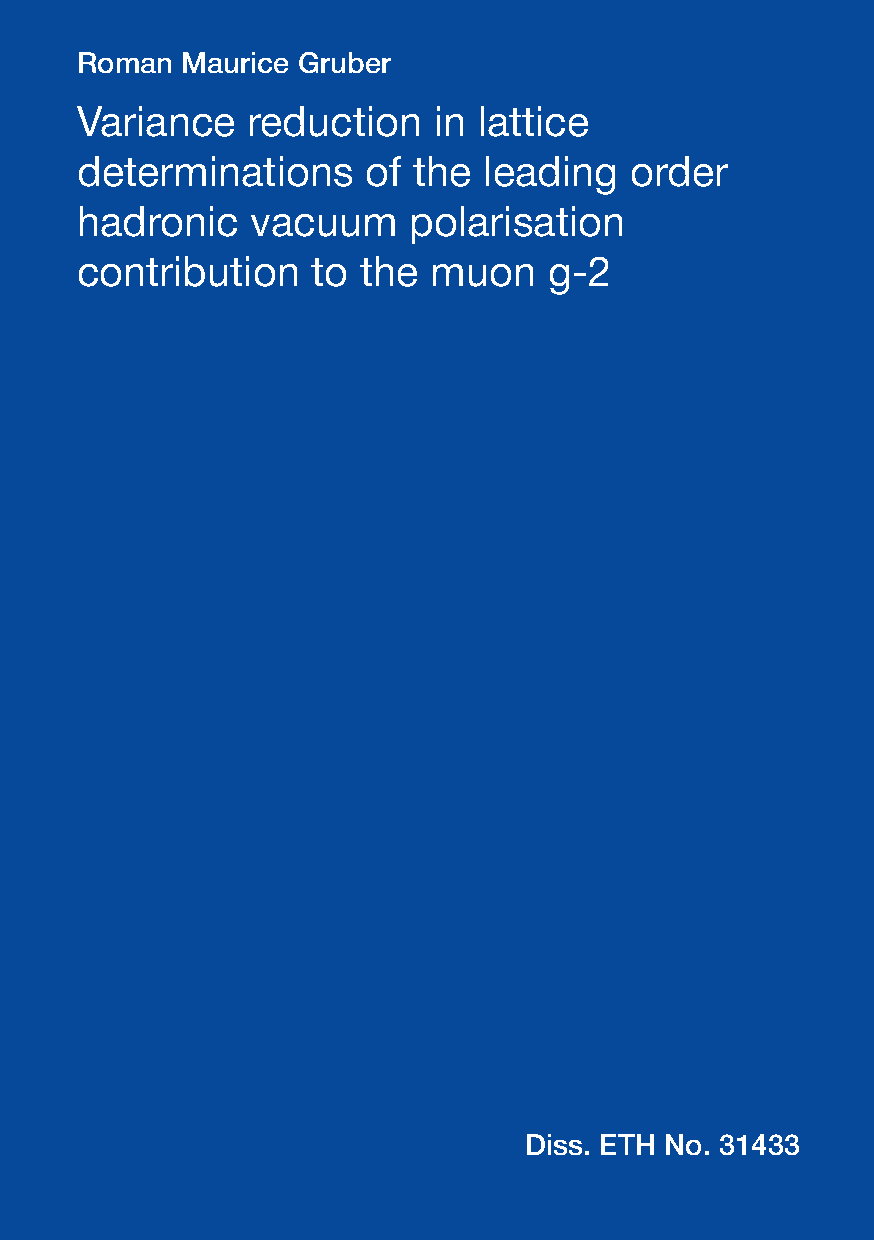
\includepdf[pages={1,{}}]{cover/crop/cover_front.pdf}
\cleardoublepage\setcounter{page}{1}

%
% Some citations that should ALWAYS be there in order
%
\nociteOwn{mglma}
\nociteOwn{qcd_qed_paola}
\nociteOwn{pasc23}
\nociteOwn{pasc24}
\nociteOwn{lattice21:master_thesis}
\nociteOwn{lattice23:lma}
\nociteOwn{lattice22:paola}
\nociteOwn{lattice22:roman}
\nociteOwn{lattice22:alessandro}
\nociteOwn{lattice22:jens}
\nociteOwn{lattice24:roman}

%
% Frontmatter
%

% PYTHON: title or dirtytitlepage
\include{frontbackmatter/dirtytitlepage}

% PYTHON: title or titlepage
%*******************************************************
% Titlepage
%*******************************************************
\begin{titlepage}
	% if you want the titlepage to be centered, uncomment and fine-tune the line below (KOMA classes environment)
	%\begin{addmargin}[-1cm]{-3cm}
    \begin{center}
        \large
        \begingroup
            \spacedlowsmallcaps{Diss. ETH No. \myDissNumber}
        \endgroup

        \hfill

        \vfill

        \begingroup
            \spacedallcaps{\myTitle}
            %\spacedallcaps{\myTitleLineOne}\\
            %\spacedallcaps{\myTitleLineTwo}\\
            %\spacedallcaps{\myTitleLineThree}
        \endgroup

        \vfill

        \begingroup
            A dissertation submitted to attain the degree of \\
            \vspace{0.5em}
            \spacedlowsmallcaps{Doctor of Sciences}
            of
            \spacedlowsmallcaps{ETH Zurich} \\
            (Dr.\ sc.\ ETH Zurich)
        \endgroup

        \vfill

        \begingroup
            presented by\\
            \vspace{0.5em}
            \spacedlowsmallcaps{\myName} \\
            Dipl., Eidgenössisches Polytechnikum \\
            \vspace{0.5em}
            born on 13 February 1987 \\
            citizen of Switzerland
        \endgroup

        \vfill

        \begingroup
            accepted on the recommendation of \\
            \vspace{0.5em}
            Prof.\ Dr.\ Marina Krstić Marinković, supervisor \\
            Prof.\ Dr.\ Thomas C. Schulthess, second topical supervisor \\
            \worktodo{co-examiner}, examiner \\
            \worktodo{co-examiner}, co-examiner \\
        \endgroup

        \vfill

        \myTime%

        \vfill
    \end{center}
  %\end{addmargin}
\end{titlepage}


% PYTHON: title or titleback
\include{frontbackmatter/titleback}

% PYTHON: front or dedication or ded
\cleardoublepage%*******************************************************
% Dedication
%*******************************************************
\thispagestyle{empty}
%\phantomsection
\refstepcounter{dummy}
%\pdfbookmark[1]{Dedication}{Dedication}

\vspace*{3cm}

\begin{center}
    To \worktodo{Cheryl}
\end{center}

\medskip


% PYTHON: front or abstract
\cleardoublepage%*******************************************************
% Abstract
%*******************************************************
%\renewcommand{\abstractname}{Abstract}
\pdfbookmark[1]{Abstract}{Abstract}
\begingroup
\let\clearpage\relax
\let\cleardoublepage\relax
\let\cleardoublepage\relax

\chapter*{Abstract}

The \openqxd codebase was interfaced to \quda, enabling utilization of modern GPU-based compute clusters in the observable evaluation phase of computational lattice field theory, where solves of the Dirac equation can be offloaded to \quda.
Features like spatial \Cstar boundary conditions and the QCD+QED Wilson-Clover Dirac operator were implemented directly in \quda.
Special emphasis was taken on versatility and convenience on the application level for interaction with the interface allowing hybrid and heterogeneous workloads.
Further focus was drawn on efficient performance on a variety of modern compute infrastructure culminating in a range of scaling studies.
Code robustness can be guaranteed by a CI/CD pipeline running directly on production machines at CSCS.

A novel variance reduction method called multigrid low-mode averaging was developed and investigated.
The method is inspired by solver preconditioning methods such as multigrid and inexact deflation, where efficient low-mode subspaces are generated by exploiting local coherence of low modes.
Since traditional methods show disadvantageous quadratic scaling in the lattice volume making them prohibitively expensive as volumes increase, the numerical study focuses on the volume scaling behavior of the proposed method.
The main result of this thesis shows linear volume scaling of the new method, while achieving constant variance reduction with a constant number of low modes of \num{50} on all investigated lattices.
This renders the method a promising candidate for observables suffering from the signal-to-noise ratio problem on large physical point lattices near the chiral limit.

\endgroup

\cleardoublepage%

\begingroup
\let\clearpage\relax
\let\cleardoublepage\relax
\let\cleardoublepage\relax

\begin{otherlanguage}{ngerman}
\pdfbookmark[1]{Zusammenfassung}{Zusammenfassung}
\chapter*{Zusammenfassung}

Das Simulationsprogramm \openqxd wurde mit einem Interface zu \quda ausgestattet, womit moderne GPU-basierte Rechencluster für die Observablenberechnung in der computergestützten Gitterfeldtheorie genutzt werden können, insbesondere durch das Auslagern der Lösung der Diracgleichung an \quda.
Funkionalitäten sowie raumliche \Cstar Randbedingungen sowie der QCD+QED Wilson-Clover Dirac Operator wurden direkt in \quda implementiert.
Besonderer Wert wurde auf Vielseitigkeit und Anwenderfreundlichekeit gelegt, um eine flexible Interaktion mit der Schnittstelle und hybride oder heterogene Arbeitlasten zu gewährleisten.
Ein weiterer Schwerpunkt wurde auf die effiziente Nutzung von moderner Recheninfrastrukturen gelegt, was in einer Reihe von Skalierungsstudien resultierte.
Die Robustheit des Codes wird durch einen CI/CD Pipeline gewährleistet, die direkt auf Produktionsmaschinen am CSCS ausgeführt wird.

Eine neue Varianzreduktionsmethode names Multigrid Low-Mode Averaging wurde entwickelt und untersucht.
Die Methode ist inspiriert durch Vorkonditionierungstechniken wie Multigrid oder inexact Deflation, bei denen effizient Unterräume assoziiert zu niedrigen Moden mittels Ausnutzung lokaler Kohärenz konstruiert werden.
Da herkömmliche Verfahren eine ungünstige quadratische Skalierung im Gittervolumen aufweisen und bei grossen Volumina schnell undurchführbar werden, konzentriert sich die numerische Untersuchung auf das Volumen-Skalierungsverhalten der neuen Methode.
%Das Hauptergebnis dieser Arbeit zeigt, dass die neue Methode eine lineare Volumenskalierung erreicht und gleichzeitig die Varianzreduktion konstant halten kann bei einer konstanten Anzahl von \num{50} niegriger Moden auf allen untersuchten Gittern.
Das Hauptergebnis dieser Arbeit zeigt, dass die neue Methode eine lineare Volumenskalierung erreicht und gleichzeitig die Varianzreduktion bei einer konstanten Anzahl von \num{50} niedriger Moden auf allen untersuchten Gittern konstant halten kann.

Dies macht sie zu einem vielversprechendem Kandidaten für Observablen, die unter dem Signal-zu-Rausch-Verhältnis leiden, speziell auf grossen physikalischen Gittern nahe des chiralen Limits.

\end{otherlanguage}

\endgroup

\vfill

% PYTHON: front or doo or declaration or dec
\cleardoublepage%*******************************************************
% Decalration of Originality
%*******************************************************
\pdfbookmark[1]{Declaration of Originality}{Declaration of Originality}
\begingroup
\let\clearpage\relax
\let\cleardoublepage\relax
\let\cleardoublepage\relax

\chapter*{Declaration of Originality}

I, Roman Gruber, declare hereby that the contents of this thesis are based on my research at ETH Zürich.
The work and results presented in this document have been produced by me in conjunction with my supervisor Prof. Marina Krstić Marinković, other members of the Computational Lattice Field Theory research group in Zürich, members associated to the PASC project~\cite{online:pasc2021} and members of the \RCstar collaboration.
I confirm that I have not submitted any part of this work for another degree or qualification anywhere else.

The contents of \cref{part:gpu} are partly relying on ref.~\citeOwn{pasc24} which is currently unpublished, but we plan to publish in the near future.
Small parts where published in the conference proceeding ref.~\citeOwn{lattice24:roman}.

The contents of \cref{part:variance} are based on an early and incomplete conference proceeding ref.~\citeOwn{lattice23:lma}, whereas most of the results rely on ref.~\citeOwn{mglma}.
Some of the plots are taken from ref.~\citeOwn{mglma}, if so it is indicated in the captions.

\endgroup


% PYTHON: front or acknowledgments or ack
\cleardoublepage%*******************************************************
% Acknowledgments
%*******************************************************
\pdfbookmark[1]{Acknowledgements}{acknowledgements}

\bigskip

\begingroup
\let\clearpage\relax
\let\cleardoublepage\relax
\let\cleardoublepage\relax
\chapter*{Acknowledgements}

\def\thanks#1{%
\begingroup
\leftskip1em
\noindent #1
\par
\endgroup
}

%\worktodo{
%* Marina who has introduced me to this vast research field of possibilities
%* Schulthess introduced me to marina for my master thesis and served as my second supervisor
%* ZH people
%* RCstar people
%* Cheryl for her continuous support and for fighting through an early version of this document (voluntarily!).
%* countless nights with coffee
%* my cats for chasing the mouse cursor or sitting directly onto my keyboard (footnote: all errors in this document arose through this, I attribute all errors in this document to them) or zoom-bombing me repeatedly
%}

%\worktodo{I would like to thank \dots}

First and foremost, I would like to thank my supervisor, Prof. Marina Marinković, for her continuous guidance, patience and for introducing me to this vast research field with its many possibilities.
I appreciate the freedom and trust she gave me to explore my own ideas.

I thank Prof. Thomas Schulthess for introducing me to Marina during my master thesis and for serving as my second supervisor.

The people from the research group in Zürich, I would like to thank for their inputs and constructive feedback, specially Tim Harris for countless discussions about noise and for showing me repeatedly that variances of diagrams are diagrams themselves.

I thank the members of the \RCstar collaboration for accepting me as one of their own, giving me the opportunity to integrate my research into the broader perspective of its scientific goals and for enduring my way-too-long presentations on various topics.

My girlfriend Cheryl supported me all the way through, I am grateful to that.
She fought through an early unreadable version of this document\footnote{Voluntarily!}.

This work would not have been possible without my cats; my emotional support animals.
I thank them for distracting me, chasing my mouse cursor, zoom-bombing me or sitting directly on my keyboardddddddddddddddd\footnote{This led to some of my best results, but I attribute all errors in this document to them alone.}.
They were my constant companions through countless coffee-fueled days and nights.

I am grateful to Richard Brower, Kate Clark, Carlton De Tar, Aida El-Khadra, Leonardo Giusti, Steven Gottlieb, Bartosz Kostrzewa, Simon Kuberski, Christoph Lehner, Martin Lüscher and Mathias Wagner for insightful discussions at conferences or visits.

The support for the PASC 2021-2024 project ``Efficient QCD+QED Simulations with openQ*D software''~\cite{online:pasc2021} is gratefully acknowledged.

I acknowledge the access to Piz Daint and Daint Alps at the Swiss National Supercomputing Centre, Switzerland under the ETHZ’s share with the project IDs c21, ch16, eth8, go21 and s1196.

I gratefully acknowledge the Gauss Centre for Supercomputing e.V. (www.gauss-centre.eu) for funding this project by providing computing time on the GCS Supercomputer JUWELS~\cite{juwels} at Jülich Supercomputing Centre (JSC). 

I acknowledge the EuroHPC Joint Undertaking for awarding this project access to the EuroHPC supercomputer LUMI, hosted by CSC (Finland) and the LUMI consortium through a EuroHPC Regular Access call.

I acknowledge the EuroHPC Joint Undertaking for awarding this project access to the EuroHPC supercomputer LEONARDO, hosted by CINECA (Italy) and the LEONARDO consortium through an EuroHPC Regular Access call.

% \worktodo{
% This work was supported by the  Platform for Advanced Scientific Computing (PASC) project "name of the project". \cite{online:pasc2021}"
% * old daint
% * daint alps
% * LUMI-C
% * JUWELS
% * Leonardo
% }

Finally, I want to explicitly clarify how and to what extent I have used generative AI technologies in the writing of this thesis.
Mainly it has been used for three tasks:
(1) Asking clarification questions about technical details (e.g. the role of the SW-term in the Wilson Dirac operator);
(2) Suggestion of reformulations of draft paragraphs. 
I never copied such rewritings, but eventually used them as basis for refactoring pieces of text.
Although there might be very few sentences in this document which are direct copies;
(3) Help ensure completeness when reviewing known technology or algorithms (e.g. a list of variance reduction methods).
Responses were used as a basis.

%or similar\footnote{I even asked the AI how to cite generative AI tools properly in a PhD thesis which is a little ironic. It said one sentence is enough.}

\endgroup


\pagestyle{scrheadings}

% PYTHON: front or toc
\cleardoublepage%*******************************************************
% Table of Contents
%*******************************************************
%\phantomsection
\refstepcounter{dummy}
\renewcommand*\contentsname{Table of Contents}
\pdfbookmark[1]{\contentsname}{tableofcontents}
\setcounter{tocdepth}{1} % <-- 2 includes up to subsections in the ToC
\setcounter{secnumdepth}{2} % <-- 3 numbers up to subsubsections
\manualmark%
\markboth{\spacedlowsmallcaps{\contentsname}}{\spacedlowsmallcaps{\contentsname}}
\tableofcontents
\automark[section]{chapter}
\renewcommand{\chaptermark}[1]{\markboth{\spacedlowsmallcaps{#1}}{\spacedlowsmallcaps{#1}}}
\renewcommand{\sectionmark}[1]{\markright{\thesection\enspace\spacedlowsmallcaps{#1}}}
%*******************************************************
% List of Figures and of the Tables
%*******************************************************
\clearpage

\begingroup
\let\clearpage\relax
\let\cleardoublepage\relax
\let\cleardoublepage\relax
%*******************************************************
% List of Figures
%*******************************************************
%\phantomsection
% \refstepcounter{dummy}
%\addcontentsline{toc}{chapter}{\listfigurename}
% \pdfbookmark[1]{\listfigurename}{lof}
% \listoffigures

% \vspace{8ex}

%*******************************************************
% List of Tables
%*******************************************************
%\phantomsection
% \refstepcounter{dummy}
%\addcontentsline{toc}{chapter}{\listtablename}
% \pdfbookmark[1]{\listtablename}{lot}
% \listoftables

% \vspace{8ex}
% \newpage

%*******************************************************
% List of Listings
%*******************************************************
  %\phantomsection
%\refstepcounter{dummy}
%\addcontentsline{toc}{chapter}{\lstlistlistingname}
%\pdfbookmark[1]{\lstlistlistingname}{lol}
%\lstlistoflistings%

%\vspace{8ex}

\endgroup


%
% Mainmatter
%

% PYTHON: main or notation
\cleardoublepage\pagenumbering{arabic}%
\def\dir{chapters/00-notation}
\chapter{QUDA}
\label{ch:p1:quda}

QUDA \cite{QUDApaper} is a library written in CUDA C++ that contains a suite of efficient kernels and solvers to implement lattice QCD simulations (the current release version 1.1.0 complies with the C++14 and 17 standards). It is thus natural that QCD fields are represented by objects, and the pointers to the fields' values are accessible via their objects.

% making use of the modern C++ standards, an  with  making use of the object paradigm and a high degree of abstraction.
% \todo{exact standard?: by checking the CMakeFiles, QUDA v.1.0 got C++11 or 14, in v.1.1.0 needs C++14 or 17 (ref: \code{https://github.com/search?q=repo\%3Alattice\%2Fquda+c\%2B\%2B17\&type=code}, and 
% }, 

A spinor field is represented by an instance of \code{ColorSpinorField}, a gauge field by \code{GaugeField} and a clover field as \code{CloverField}, all of which inherit from the \code{LatticeField} class. The different degrees of freedom are realised in the inheriting classes. The actual numbers are accessible via a pointer whose accessor is called \code{data()}.

QUDA is highly optimized to run on multiple GPUs, specifically on NVIDIA and AMD cards. In addition, it offers a multi-threading backend.


% PYTHON: main or intro or introduction
\cleardoublepage%\pagenumbering{arabic}%
\def\dir{chapters/01-introduction}
\chapter{QUDA}
\label{ch:p1:quda}

QUDA \cite{QUDApaper} is a library written in CUDA C++ that contains a suite of efficient kernels and solvers to implement lattice QCD simulations (the current release version 1.1.0 complies with the C++14 and 17 standards). It is thus natural that QCD fields are represented by objects, and the pointers to the fields' values are accessible via their objects.

% making use of the modern C++ standards, an  with  making use of the object paradigm and a high degree of abstraction.
% \todo{exact standard?: by checking the CMakeFiles, QUDA v.1.0 got C++11 or 14, in v.1.1.0 needs C++14 or 17 (ref: \code{https://github.com/search?q=repo\%3Alattice\%2Fquda+c\%2B\%2B17\&type=code}, and 
% }, 

A spinor field is represented by an instance of \code{ColorSpinorField}, a gauge field by \code{GaugeField} and a clover field as \code{CloverField}, all of which inherit from the \code{LatticeField} class. The different degrees of freedom are realised in the inheriting classes. The actual numbers are accessible via a pointer whose accessor is called \code{data()}.

QUDA is highly optimized to run on multiple GPUs, specifically on NVIDIA and AMD cards. In addition, it offers a multi-threading backend.


% Include some blind text
%\Blinddocument

% PYTHON: deprecated and (main or lit or review)
%\cleardoublepage%
%\def\dir{chapters/02-literature-review}
%\chapter{QUDA}
\label{ch:p1:quda}

QUDA \cite{QUDApaper} is a library written in CUDA C++ that contains a suite of efficient kernels and solvers to implement lattice QCD simulations (the current release version 1.1.0 complies with the C++14 and 17 standards). It is thus natural that QCD fields are represented by objects, and the pointers to the fields' values are accessible via their objects.

% making use of the modern C++ standards, an  with  making use of the object paradigm and a high degree of abstraction.
% \todo{exact standard?: by checking the CMakeFiles, QUDA v.1.0 got C++11 or 14, in v.1.1.0 needs C++14 or 17 (ref: \code{https://github.com/search?q=repo\%3Alattice\%2Fquda+c\%2B\%2B17\&type=code}, and 
% }, 

A spinor field is represented by an instance of \code{ColorSpinorField}, a gauge field by \code{GaugeField} and a clover field as \code{CloverField}, all of which inherit from the \code{LatticeField} class. The different degrees of freedom are realised in the inheriting classes. The actual numbers are accessible via a pointer whose accessor is called \code{data()}.

QUDA is highly optimized to run on multiple GPUs, specifically on NVIDIA and AMD cards. In addition, it offers a multi-threading backend.


% Part I: GPU Port
% PYTHON: main or part1 or p1label or label
\part{GPU Porting of Dirac Solvers}
\label{part:gpu}

% PYTHON: main or part1 or part1_introduction or part1_intro or p1intro
\cleardoublepage%
\def\dir{chapters/part-1/01-introduction}
\chapter{QUDA}
\label{ch:p1:quda}

QUDA \cite{QUDApaper} is a library written in CUDA C++ that contains a suite of efficient kernels and solvers to implement lattice QCD simulations (the current release version 1.1.0 complies with the C++14 and 17 standards). It is thus natural that QCD fields are represented by objects, and the pointers to the fields' values are accessible via their objects.

% making use of the modern C++ standards, an  with  making use of the object paradigm and a high degree of abstraction.
% \todo{exact standard?: by checking the CMakeFiles, QUDA v.1.0 got C++11 or 14, in v.1.1.0 needs C++14 or 17 (ref: \code{https://github.com/search?q=repo\%3Alattice\%2Fquda+c\%2B\%2B17\&type=code}, and 
% }, 

A spinor field is represented by an instance of \code{ColorSpinorField}, a gauge field by \code{GaugeField} and a clover field as \code{CloverField}, all of which inherit from the \code{LatticeField} class. The different degrees of freedom are realised in the inheriting classes. The actual numbers are accessible via a pointer whose accessor is called \code{data()}.

QUDA is highly optimized to run on multiple GPUs, specifically on NVIDIA and AMD cards. In addition, it offers a multi-threading backend.


% PYTHON: main or part1 or openqxd or openqcd
\cleardoublepage%
\def\dir{chapters/part-1/02-openqxd}
\chapter{QUDA}
\label{ch:p1:quda}

QUDA \cite{QUDApaper} is a library written in CUDA C++ that contains a suite of efficient kernels and solvers to implement lattice QCD simulations (the current release version 1.1.0 complies with the C++14 and 17 standards). It is thus natural that QCD fields are represented by objects, and the pointers to the fields' values are accessible via their objects.

% making use of the modern C++ standards, an  with  making use of the object paradigm and a high degree of abstraction.
% \todo{exact standard?: by checking the CMakeFiles, QUDA v.1.0 got C++11 or 14, in v.1.1.0 needs C++14 or 17 (ref: \code{https://github.com/search?q=repo\%3Alattice\%2Fquda+c\%2B\%2B17\&type=code}, and 
% }, 

A spinor field is represented by an instance of \code{ColorSpinorField}, a gauge field by \code{GaugeField} and a clover field as \code{CloverField}, all of which inherit from the \code{LatticeField} class. The different degrees of freedom are realised in the inheriting classes. The actual numbers are accessible via a pointer whose accessor is called \code{data()}.

QUDA is highly optimized to run on multiple GPUs, specifically on NVIDIA and AMD cards. In addition, it offers a multi-threading backend.


% PYTHON: main or part1 or quda
\cleardoublepage%
\def\dir{chapters/part-1/03-quda}
\chapter{QUDA}
\label{ch:p1:quda}

QUDA \cite{QUDApaper} is a library written in CUDA C++ that contains a suite of efficient kernels and solvers to implement lattice QCD simulations (the current release version 1.1.0 complies with the C++14 and 17 standards). It is thus natural that QCD fields are represented by objects, and the pointers to the fields' values are accessible via their objects.

% making use of the modern C++ standards, an  with  making use of the object paradigm and a high degree of abstraction.
% \todo{exact standard?: by checking the CMakeFiles, QUDA v.1.0 got C++11 or 14, in v.1.1.0 needs C++14 or 17 (ref: \code{https://github.com/search?q=repo\%3Alattice\%2Fquda+c\%2B\%2B17\&type=code}, and 
% }, 

A spinor field is represented by an instance of \code{ColorSpinorField}, a gauge field by \code{GaugeField} and a clover field as \code{CloverField}, all of which inherit from the \code{LatticeField} class. The different degrees of freedom are realised in the inheriting classes. The actual numbers are accessible via a pointer whose accessor is called \code{data()}.

QUDA is highly optimized to run on multiple GPUs, specifically on NVIDIA and AMD cards. In addition, it offers a multi-threading backend.


% PYTHON: main or part1 or interface or int
\cleardoublepage%
\def\dir{chapters/part-1/04-interface}
\chapter{QUDA}
\label{ch:p1:quda}

QUDA \cite{QUDApaper} is a library written in CUDA C++ that contains a suite of efficient kernels and solvers to implement lattice QCD simulations (the current release version 1.1.0 complies with the C++14 and 17 standards). It is thus natural that QCD fields are represented by objects, and the pointers to the fields' values are accessible via their objects.

% making use of the modern C++ standards, an  with  making use of the object paradigm and a high degree of abstraction.
% \todo{exact standard?: by checking the CMakeFiles, QUDA v.1.0 got C++11 or 14, in v.1.1.0 needs C++14 or 17 (ref: \code{https://github.com/search?q=repo\%3Alattice\%2Fquda+c\%2B\%2B17\&type=code}, and 
% }, 

A spinor field is represented by an instance of \code{ColorSpinorField}, a gauge field by \code{GaugeField} and a clover field as \code{CloverField}, all of which inherit from the \code{LatticeField} class. The different degrees of freedom are realised in the inheriting classes. The actual numbers are accessible via a pointer whose accessor is called \code{data()}.

QUDA is highly optimized to run on multiple GPUs, specifically on NVIDIA and AMD cards. In addition, it offers a multi-threading backend.


% PYTHON: main or part1 or (developing or dev)
\cleardoublepage%
\def\dir{chapters/part-1/05-developing}
\chapter{QUDA}
\label{ch:p1:quda}

QUDA \cite{QUDApaper} is a library written in CUDA C++ that contains a suite of efficient kernels and solvers to implement lattice QCD simulations (the current release version 1.1.0 complies with the C++14 and 17 standards). It is thus natural that QCD fields are represented by objects, and the pointers to the fields' values are accessible via their objects.

% making use of the modern C++ standards, an  with  making use of the object paradigm and a high degree of abstraction.
% \todo{exact standard?: by checking the CMakeFiles, QUDA v.1.0 got C++11 or 14, in v.1.1.0 needs C++14 or 17 (ref: \code{https://github.com/search?q=repo\%3Alattice\%2Fquda+c\%2B\%2B17\&type=code}, and 
% }, 

A spinor field is represented by an instance of \code{ColorSpinorField}, a gauge field by \code{GaugeField} and a clover field as \code{CloverField}, all of which inherit from the \code{LatticeField} class. The different degrees of freedom are realised in the inheriting classes. The actual numbers are accessible via a pointer whose accessor is called \code{data()}.

QUDA is highly optimized to run on multiple GPUs, specifically on NVIDIA and AMD cards. In addition, it offers a multi-threading backend.


% PYTHON: deprecated and (main or part1 or (building or build))
%\cleardoublepage%
%\def\dir{chapters/part-1/00-deprecated_06-building}
%\chapter{QUDA}
\label{ch:p1:quda}

QUDA \cite{QUDApaper} is a library written in CUDA C++ that contains a suite of efficient kernels and solvers to implement lattice QCD simulations (the current release version 1.1.0 complies with the C++14 and 17 standards). It is thus natural that QCD fields are represented by objects, and the pointers to the fields' values are accessible via their objects.

% making use of the modern C++ standards, an  with  making use of the object paradigm and a high degree of abstraction.
% \todo{exact standard?: by checking the CMakeFiles, QUDA v.1.0 got C++11 or 14, in v.1.1.0 needs C++14 or 17 (ref: \code{https://github.com/search?q=repo\%3Alattice\%2Fquda+c\%2B\%2B17\&type=code}, and 
% }, 

A spinor field is represented by an instance of \code{ColorSpinorField}, a gauge field by \code{GaugeField} and a clover field as \code{CloverField}, all of which inherit from the \code{LatticeField} class. The different degrees of freedom are realised in the inheriting classes. The actual numbers are accessible via a pointer whose accessor is called \code{data()}.

QUDA is highly optimized to run on multiple GPUs, specifically on NVIDIA and AMD cards. In addition, it offers a multi-threading backend.


% PYTHON: deprecated and (main or part1 or (running or run))
%\cleardoublepage%
%\def\dir{chapters/part-1/00-deprecated_07-running}
%\chapter{QUDA}
\label{ch:p1:quda}

QUDA \cite{QUDApaper} is a library written in CUDA C++ that contains a suite of efficient kernels and solvers to implement lattice QCD simulations (the current release version 1.1.0 complies with the C++14 and 17 standards). It is thus natural that QCD fields are represented by objects, and the pointers to the fields' values are accessible via their objects.

% making use of the modern C++ standards, an  with  making use of the object paradigm and a high degree of abstraction.
% \todo{exact standard?: by checking the CMakeFiles, QUDA v.1.0 got C++11 or 14, in v.1.1.0 needs C++14 or 17 (ref: \code{https://github.com/search?q=repo\%3Alattice\%2Fquda+c\%2B\%2B17\&type=code}, and 
% }, 

A spinor field is represented by an instance of \code{ColorSpinorField}, a gauge field by \code{GaugeField} and a clover field as \code{CloverField}, all of which inherit from the \code{LatticeField} class. The different degrees of freedom are realised in the inheriting classes. The actual numbers are accessible via a pointer whose accessor is called \code{data()}.

QUDA is highly optimized to run on multiple GPUs, specifically on NVIDIA and AMD cards. In addition, it offers a multi-threading backend.


% PYTHON: main or part1 or (performance or perf)
\cleardoublepage%
\def\dir{chapters/part-1/08-performance}
\chapter{QUDA}
\label{ch:p1:quda}

QUDA \cite{QUDApaper} is a library written in CUDA C++ that contains a suite of efficient kernels and solvers to implement lattice QCD simulations (the current release version 1.1.0 complies with the C++14 and 17 standards). It is thus natural that QCD fields are represented by objects, and the pointers to the fields' values are accessible via their objects.

% making use of the modern C++ standards, an  with  making use of the object paradigm and a high degree of abstraction.
% \todo{exact standard?: by checking the CMakeFiles, QUDA v.1.0 got C++11 or 14, in v.1.1.0 needs C++14 or 17 (ref: \code{https://github.com/search?q=repo\%3Alattice\%2Fquda+c\%2B\%2B17\&type=code}, and 
% }, 

A spinor field is represented by an instance of \code{ColorSpinorField}, a gauge field by \code{GaugeField} and a clover field as \code{CloverField}, all of which inherit from the \code{LatticeField} class. The different degrees of freedom are realised in the inheriting classes. The actual numbers are accessible via a pointer whose accessor is called \code{data()}.

QUDA is highly optimized to run on multiple GPUs, specifically on NVIDIA and AMD cards. In addition, it offers a multi-threading backend.


% PYTHON: main or part1 or (cicd)
\cleardoublepage%
\def\dir{chapters/part-1/09-cicd}
\chapter{QUDA}
\label{ch:p1:quda}

QUDA \cite{QUDApaper} is a library written in CUDA C++ that contains a suite of efficient kernels and solvers to implement lattice QCD simulations (the current release version 1.1.0 complies with the C++14 and 17 standards). It is thus natural that QCD fields are represented by objects, and the pointers to the fields' values are accessible via their objects.

% making use of the modern C++ standards, an  with  making use of the object paradigm and a high degree of abstraction.
% \todo{exact standard?: by checking the CMakeFiles, QUDA v.1.0 got C++11 or 14, in v.1.1.0 needs C++14 or 17 (ref: \code{https://github.com/search?q=repo\%3Alattice\%2Fquda+c\%2B\%2B17\&type=code}, and 
% }, 

A spinor field is represented by an instance of \code{ColorSpinorField}, a gauge field by \code{GaugeField} and a clover field as \code{CloverField}, all of which inherit from the \code{LatticeField} class. The different degrees of freedom are realised in the inheriting classes. The actual numbers are accessible via a pointer whose accessor is called \code{data()}.

QUDA is highly optimized to run on multiple GPUs, specifically on NVIDIA and AMD cards. In addition, it offers a multi-threading backend.


% PYTHON: main or part1 or (memory_manager or mm)
\cleardoublepage%
\def\dir{chapters/part-1/10-memory-manager}
\chapter{QUDA}
\label{ch:p1:quda}

QUDA \cite{QUDApaper} is a library written in CUDA C++ that contains a suite of efficient kernels and solvers to implement lattice QCD simulations (the current release version 1.1.0 complies with the C++14 and 17 standards). It is thus natural that QCD fields are represented by objects, and the pointers to the fields' values are accessible via their objects.

% making use of the modern C++ standards, an  with  making use of the object paradigm and a high degree of abstraction.
% \todo{exact standard?: by checking the CMakeFiles, QUDA v.1.0 got C++11 or 14, in v.1.1.0 needs C++14 or 17 (ref: \code{https://github.com/search?q=repo\%3Alattice\%2Fquda+c\%2B\%2B17\&type=code}, and 
% }, 

A spinor field is represented by an instance of \code{ColorSpinorField}, a gauge field by \code{GaugeField} and a clover field as \code{CloverField}, all of which inherit from the \code{LatticeField} class. The different degrees of freedom are realised in the inheriting classes. The actual numbers are accessible via a pointer whose accessor is called \code{data()}.

QUDA is highly optimized to run on multiple GPUs, specifically on NVIDIA and AMD cards. In addition, it offers a multi-threading backend.


% PYTHON: main or part1 or (conclusions or concl or p1concl)
\cleardoublepage%
\def\dir{chapters/part-1/11-conclusions}
\chapter{QUDA}
\label{ch:p1:quda}

QUDA \cite{QUDApaper} is a library written in CUDA C++ that contains a suite of efficient kernels and solvers to implement lattice QCD simulations (the current release version 1.1.0 complies with the C++14 and 17 standards). It is thus natural that QCD fields are represented by objects, and the pointers to the fields' values are accessible via their objects.

% making use of the modern C++ standards, an  with  making use of the object paradigm and a high degree of abstraction.
% \todo{exact standard?: by checking the CMakeFiles, QUDA v.1.0 got C++11 or 14, in v.1.1.0 needs C++14 or 17 (ref: \code{https://github.com/search?q=repo\%3Alattice\%2Fquda+c\%2B\%2B17\&type=code}, and 
% }, 

A spinor field is represented by an instance of \code{ColorSpinorField}, a gauge field by \code{GaugeField} and a clover field as \code{CloverField}, all of which inherit from the \code{LatticeField} class. The different degrees of freedom are realised in the inheriting classes. The actual numbers are accessible via a pointer whose accessor is called \code{data()}.

QUDA is highly optimized to run on multiple GPUs, specifically on NVIDIA and AMD cards. In addition, it offers a multi-threading backend.


% Part I: MGLMA
% PYTHON: main or part2 or p2label or label
\part{Variance Reduction for Two-Point Functions}
\label{part:variance}

% PYTHON: main or part2 or part2_introduction or part2_intro or p2intro
\cleardoublepage%
\def\dir{chapters/part-2/01-introduction}
\chapter{QUDA}
\label{ch:p1:quda}

QUDA \cite{QUDApaper} is a library written in CUDA C++ that contains a suite of efficient kernels and solvers to implement lattice QCD simulations (the current release version 1.1.0 complies with the C++14 and 17 standards). It is thus natural that QCD fields are represented by objects, and the pointers to the fields' values are accessible via their objects.

% making use of the modern C++ standards, an  with  making use of the object paradigm and a high degree of abstraction.
% \todo{exact standard?: by checking the CMakeFiles, QUDA v.1.0 got C++11 or 14, in v.1.1.0 needs C++14 or 17 (ref: \code{https://github.com/search?q=repo\%3Alattice\%2Fquda+c\%2B\%2B17\&type=code}, and 
% }, 

A spinor field is represented by an instance of \code{ColorSpinorField}, a gauge field by \code{GaugeField} and a clover field as \code{CloverField}, all of which inherit from the \code{LatticeField} class. The different degrees of freedom are realised in the inheriting classes. The actual numbers are accessible via a pointer whose accessor is called \code{data()}.

QUDA is highly optimized to run on multiple GPUs, specifically on NVIDIA and AMD cards. In addition, it offers a multi-threading backend.


% PYTHON: main or part2 or two_pt_corr or 2pt or two_pt
\cleardoublepage%
\def\dir{chapters/part-2/02-two-pt-corr}
\chapter{QUDA}
\label{ch:p1:quda}

QUDA \cite{QUDApaper} is a library written in CUDA C++ that contains a suite of efficient kernels and solvers to implement lattice QCD simulations (the current release version 1.1.0 complies with the C++14 and 17 standards). It is thus natural that QCD fields are represented by objects, and the pointers to the fields' values are accessible via their objects.

% making use of the modern C++ standards, an  with  making use of the object paradigm and a high degree of abstraction.
% \todo{exact standard?: by checking the CMakeFiles, QUDA v.1.0 got C++11 or 14, in v.1.1.0 needs C++14 or 17 (ref: \code{https://github.com/search?q=repo\%3Alattice\%2Fquda+c\%2B\%2B17\&type=code}, and 
% }, 

A spinor field is represented by an instance of \code{ColorSpinorField}, a gauge field by \code{GaugeField} and a clover field as \code{CloverField}, all of which inherit from the \code{LatticeField} class. The different degrees of freedom are realised in the inheriting classes. The actual numbers are accessible via a pointer whose accessor is called \code{data()}.

QUDA is highly optimized to run on multiple GPUs, specifically on NVIDIA and AMD cards. In addition, it offers a multi-threading backend.


% PYTHON: main or part2 or lma
\cleardoublepage%
\def\dir{chapters/part-2/03-lma}
\chapter{QUDA}
\label{ch:p1:quda}

QUDA \cite{QUDApaper} is a library written in CUDA C++ that contains a suite of efficient kernels and solvers to implement lattice QCD simulations (the current release version 1.1.0 complies with the C++14 and 17 standards). It is thus natural that QCD fields are represented by objects, and the pointers to the fields' values are accessible via their objects.

% making use of the modern C++ standards, an  with  making use of the object paradigm and a high degree of abstraction.
% \todo{exact standard?: by checking the CMakeFiles, QUDA v.1.0 got C++11 or 14, in v.1.1.0 needs C++14 or 17 (ref: \code{https://github.com/search?q=repo\%3Alattice\%2Fquda+c\%2B\%2B17\&type=code}, and 
% }, 

A spinor field is represented by an instance of \code{ColorSpinorField}, a gauge field by \code{GaugeField} and a clover field as \code{CloverField}, all of which inherit from the \code{LatticeField} class. The different degrees of freedom are realised in the inheriting classes. The actual numbers are accessible via a pointer whose accessor is called \code{data()}.

QUDA is highly optimized to run on multiple GPUs, specifically on NVIDIA and AMD cards. In addition, it offers a multi-threading backend.


% PYTHON: main or part2 or subspace_deflation or subspace or sd
\cleardoublepage%
\def\dir{chapters/part-2/04-subspace-deflation}
\chapter{QUDA}
\label{ch:p1:quda}

QUDA \cite{QUDApaper} is a library written in CUDA C++ that contains a suite of efficient kernels and solvers to implement lattice QCD simulations (the current release version 1.1.0 complies with the C++14 and 17 standards). It is thus natural that QCD fields are represented by objects, and the pointers to the fields' values are accessible via their objects.

% making use of the modern C++ standards, an  with  making use of the object paradigm and a high degree of abstraction.
% \todo{exact standard?: by checking the CMakeFiles, QUDA v.1.0 got C++11 or 14, in v.1.1.0 needs C++14 or 17 (ref: \code{https://github.com/search?q=repo\%3Alattice\%2Fquda+c\%2B\%2B17\&type=code}, and 
% }, 

A spinor field is represented by an instance of \code{ColorSpinorField}, a gauge field by \code{GaugeField} and a clover field as \code{CloverField}, all of which inherit from the \code{LatticeField} class. The different degrees of freedom are realised in the inheriting classes. The actual numbers are accessible via a pointer whose accessor is called \code{data()}.

QUDA is highly optimized to run on multiple GPUs, specifically on NVIDIA and AMD cards. In addition, it offers a multi-threading backend.


% PYTHON: main or part2 or localcoherence or lc
\cleardoublepage%
\def\dir{chapters/part-2/05-local-coherence}
\chapter{QUDA}
\label{ch:p1:quda}

QUDA \cite{QUDApaper} is a library written in CUDA C++ that contains a suite of efficient kernels and solvers to implement lattice QCD simulations (the current release version 1.1.0 complies with the C++14 and 17 standards). It is thus natural that QCD fields are represented by objects, and the pointers to the fields' values are accessible via their objects.

% making use of the modern C++ standards, an  with  making use of the object paradigm and a high degree of abstraction.
% \todo{exact standard?: by checking the CMakeFiles, QUDA v.1.0 got C++11 or 14, in v.1.1.0 needs C++14 or 17 (ref: \code{https://github.com/search?q=repo\%3Alattice\%2Fquda+c\%2B\%2B17\&type=code}, and 
% }, 

A spinor field is represented by an instance of \code{ColorSpinorField}, a gauge field by \code{GaugeField} and a clover field as \code{CloverField}, all of which inherit from the \code{LatticeField} class. The different degrees of freedom are realised in the inheriting classes. The actual numbers are accessible via a pointer whose accessor is called \code{data()}.

QUDA is highly optimized to run on multiple GPUs, specifically on NVIDIA and AMD cards. In addition, it offers a multi-threading backend.


% PYTHON: main or part2 or multigrid or mg
\cleardoublepage%
\def\dir{chapters/part-2/06-multigrid}
\chapter{QUDA}
\label{ch:p1:quda}

QUDA \cite{QUDApaper} is a library written in CUDA C++ that contains a suite of efficient kernels and solvers to implement lattice QCD simulations (the current release version 1.1.0 complies with the C++14 and 17 standards). It is thus natural that QCD fields are represented by objects, and the pointers to the fields' values are accessible via their objects.

% making use of the modern C++ standards, an  with  making use of the object paradigm and a high degree of abstraction.
% \todo{exact standard?: by checking the CMakeFiles, QUDA v.1.0 got C++11 or 14, in v.1.1.0 needs C++14 or 17 (ref: \code{https://github.com/search?q=repo\%3Alattice\%2Fquda+c\%2B\%2B17\&type=code}, and 
% }, 

A spinor field is represented by an instance of \code{ColorSpinorField}, a gauge field by \code{GaugeField} and a clover field as \code{CloverField}, all of which inherit from the \code{LatticeField} class. The different degrees of freedom are realised in the inheriting classes. The actual numbers are accessible via a pointer whose accessor is called \code{data()}.

QUDA is highly optimized to run on multiple GPUs, specifically on NVIDIA and AMD cards. In addition, it offers a multi-threading backend.


% PYTHON: main or part2 or num or numerics or numerical
\cleardoublepage%
\def\dir{chapters/part-2/07-numerics}
\chapter{QUDA}
\label{ch:p1:quda}

QUDA \cite{QUDApaper} is a library written in CUDA C++ that contains a suite of efficient kernels and solvers to implement lattice QCD simulations (the current release version 1.1.0 complies with the C++14 and 17 standards). It is thus natural that QCD fields are represented by objects, and the pointers to the fields' values are accessible via their objects.

% making use of the modern C++ standards, an  with  making use of the object paradigm and a high degree of abstraction.
% \todo{exact standard?: by checking the CMakeFiles, QUDA v.1.0 got C++11 or 14, in v.1.1.0 needs C++14 or 17 (ref: \code{https://github.com/search?q=repo\%3Alattice\%2Fquda+c\%2B\%2B17\&type=code}, and 
% }, 

A spinor field is represented by an instance of \code{ColorSpinorField}, a gauge field by \code{GaugeField} and a clover field as \code{CloverField}, all of which inherit from the \code{LatticeField} class. The different degrees of freedom are realised in the inheriting classes. The actual numbers are accessible via a pointer whose accessor is called \code{data()}.

QUDA is highly optimized to run on multiple GPUs, specifically on NVIDIA and AMD cards. In addition, it offers a multi-threading backend.


% PYTHON: main or part2 or chirality or chiral or ch
\cleardoublepage%
\def\dir{chapters/part-2/08-chirality}
\chapter{QUDA}
\label{ch:p1:quda}

QUDA \cite{QUDApaper} is a library written in CUDA C++ that contains a suite of efficient kernels and solvers to implement lattice QCD simulations (the current release version 1.1.0 complies with the C++14 and 17 standards). It is thus natural that QCD fields are represented by objects, and the pointers to the fields' values are accessible via their objects.

% making use of the modern C++ standards, an  with  making use of the object paradigm and a high degree of abstraction.
% \todo{exact standard?: by checking the CMakeFiles, QUDA v.1.0 got C++11 or 14, in v.1.1.0 needs C++14 or 17 (ref: \code{https://github.com/search?q=repo\%3Alattice\%2Fquda+c\%2B\%2B17\&type=code}, and 
% }, 

A spinor field is represented by an instance of \code{ColorSpinorField}, a gauge field by \code{GaugeField} and a clover field as \code{CloverField}, all of which inherit from the \code{LatticeField} class. The different degrees of freedom are realised in the inheriting classes. The actual numbers are accessible via a pointer whose accessor is called \code{data()}.

QUDA is highly optimized to run on multiple GPUs, specifically on NVIDIA and AMD cards. In addition, it offers a multi-threading backend.


% PYTHON: main or part2 or conclusions or concl
\cleardoublepage%
\def\dir{chapters/part-2/09-conclusions}
\chapter{QUDA}
\label{ch:p1:quda}

QUDA \cite{QUDApaper} is a library written in CUDA C++ that contains a suite of efficient kernels and solvers to implement lattice QCD simulations (the current release version 1.1.0 complies with the C++14 and 17 standards). It is thus natural that QCD fields are represented by objects, and the pointers to the fields' values are accessible via their objects.

% making use of the modern C++ standards, an  with  making use of the object paradigm and a high degree of abstraction.
% \todo{exact standard?: by checking the CMakeFiles, QUDA v.1.0 got C++11 or 14, in v.1.1.0 needs C++14 or 17 (ref: \code{https://github.com/search?q=repo\%3Alattice\%2Fquda+c\%2B\%2B17\&type=code}, and 
% }, 

A spinor field is represented by an instance of \code{ColorSpinorField}, a gauge field by \code{GaugeField} and a clover field as \code{CloverField}, all of which inherit from the \code{LatticeField} class. The different degrees of freedom are realised in the inheriting classes. The actual numbers are accessible via a pointer whose accessor is called \code{data()}.

QUDA is highly optimized to run on multiple GPUs, specifically on NVIDIA and AMD cards. In addition, it offers a multi-threading backend.


% PYTHON: main or conclusion or concl
\cleardoublepage%
\def\dir{chapters/11-conclusion-outlook}
\chapter{QUDA}
\label{ch:p1:quda}

QUDA \cite{QUDApaper} is a library written in CUDA C++ that contains a suite of efficient kernels and solvers to implement lattice QCD simulations (the current release version 1.1.0 complies with the C++14 and 17 standards). It is thus natural that QCD fields are represented by objects, and the pointers to the fields' values are accessible via their objects.

% making use of the modern C++ standards, an  with  making use of the object paradigm and a high degree of abstraction.
% \todo{exact standard?: by checking the CMakeFiles, QUDA v.1.0 got C++11 or 14, in v.1.1.0 needs C++14 or 17 (ref: \code{https://github.com/search?q=repo\%3Alattice\%2Fquda+c\%2B\%2B17\&type=code}, and 
% }, 

A spinor field is represented by an instance of \code{ColorSpinorField}, a gauge field by \code{GaugeField} and a clover field as \code{CloverField}, all of which inherit from the \code{LatticeField} class. The different degrees of freedom are realised in the inheriting classes. The actual numbers are accessible via a pointer whose accessor is called \code{data()}.

QUDA is highly optimized to run on multiple GPUs, specifically on NVIDIA and AMD cards. In addition, it offers a multi-threading backend.


% Appendices
\bookmarksetup{startatroot}

\appendix

% PYTHON: back or appendix or appendices or appendixA or appA or A
\cleardoublepage%
\def\dir{chapters/appendices/A}
\chapter{QUDA}
\label{ch:p1:quda}

QUDA \cite{QUDApaper} is a library written in CUDA C++ that contains a suite of efficient kernels and solvers to implement lattice QCD simulations (the current release version 1.1.0 complies with the C++14 and 17 standards). It is thus natural that QCD fields are represented by objects, and the pointers to the fields' values are accessible via their objects.

% making use of the modern C++ standards, an  with  making use of the object paradigm and a high degree of abstraction.
% \todo{exact standard?: by checking the CMakeFiles, QUDA v.1.0 got C++11 or 14, in v.1.1.0 needs C++14 or 17 (ref: \code{https://github.com/search?q=repo\%3Alattice\%2Fquda+c\%2B\%2B17\&type=code}, and 
% }, 

A spinor field is represented by an instance of \code{ColorSpinorField}, a gauge field by \code{GaugeField} and a clover field as \code{CloverField}, all of which inherit from the \code{LatticeField} class. The different degrees of freedom are realised in the inheriting classes. The actual numbers are accessible via a pointer whose accessor is called \code{data()}.

QUDA is highly optimized to run on multiple GPUs, specifically on NVIDIA and AMD cards. In addition, it offers a multi-threading backend.


% PYTHON: back or appendix or appendices or appendixB or appB or B
\cleardoublepage%
\def\dir{chapters/appendices/B}
\chapter{QUDA}
\label{ch:p1:quda}

QUDA \cite{QUDApaper} is a library written in CUDA C++ that contains a suite of efficient kernels and solvers to implement lattice QCD simulations (the current release version 1.1.0 complies with the C++14 and 17 standards). It is thus natural that QCD fields are represented by objects, and the pointers to the fields' values are accessible via their objects.

% making use of the modern C++ standards, an  with  making use of the object paradigm and a high degree of abstraction.
% \todo{exact standard?: by checking the CMakeFiles, QUDA v.1.0 got C++11 or 14, in v.1.1.0 needs C++14 or 17 (ref: \code{https://github.com/search?q=repo\%3Alattice\%2Fquda+c\%2B\%2B17\&type=code}, and 
% }, 

A spinor field is represented by an instance of \code{ColorSpinorField}, a gauge field by \code{GaugeField} and a clover field as \code{CloverField}, all of which inherit from the \code{LatticeField} class. The different degrees of freedom are realised in the inheriting classes. The actual numbers are accessible via a pointer whose accessor is called \code{data()}.

QUDA is highly optimized to run on multiple GPUs, specifically on NVIDIA and AMD cards. In addition, it offers a multi-threading backend.


% PYTHON: back or appendix or appendices or appendixC or appC or C
\cleardoublepage%
\def\dir{chapters/appendices/C}
\chapter{QUDA}
\label{ch:p1:quda}

QUDA \cite{QUDApaper} is a library written in CUDA C++ that contains a suite of efficient kernels and solvers to implement lattice QCD simulations (the current release version 1.1.0 complies with the C++14 and 17 standards). It is thus natural that QCD fields are represented by objects, and the pointers to the fields' values are accessible via their objects.

% making use of the modern C++ standards, an  with  making use of the object paradigm and a high degree of abstraction.
% \todo{exact standard?: by checking the CMakeFiles, QUDA v.1.0 got C++11 or 14, in v.1.1.0 needs C++14 or 17 (ref: \code{https://github.com/search?q=repo\%3Alattice\%2Fquda+c\%2B\%2B17\&type=code}, and 
% }, 

A spinor field is represented by an instance of \code{ColorSpinorField}, a gauge field by \code{GaugeField} and a clover field as \code{CloverField}, all of which inherit from the \code{LatticeField} class. The different degrees of freedom are realised in the inheriting classes. The actual numbers are accessible via a pointer whose accessor is called \code{data()}.

QUDA is highly optimized to run on multiple GPUs, specifically on NVIDIA and AMD cards. In addition, it offers a multi-threading backend.


% PYTHON: back or appendix or appendices or appendixC or appD or D
\cleardoublepage%
\def\dir{chapters/appendices/D}
\chapter{QUDA}
\label{ch:p1:quda}

QUDA \cite{QUDApaper} is a library written in CUDA C++ that contains a suite of efficient kernels and solvers to implement lattice QCD simulations (the current release version 1.1.0 complies with the C++14 and 17 standards). It is thus natural that QCD fields are represented by objects, and the pointers to the fields' values are accessible via their objects.

% making use of the modern C++ standards, an  with  making use of the object paradigm and a high degree of abstraction.
% \todo{exact standard?: by checking the CMakeFiles, QUDA v.1.0 got C++11 or 14, in v.1.1.0 needs C++14 or 17 (ref: \code{https://github.com/search?q=repo\%3Alattice\%2Fquda+c\%2B\%2B17\&type=code}, and 
% }, 

A spinor field is represented by an instance of \code{ColorSpinorField}, a gauge field by \code{GaugeField} and a clover field as \code{CloverField}, all of which inherit from the \code{LatticeField} class. The different degrees of freedom are realised in the inheriting classes. The actual numbers are accessible via a pointer whose accessor is called \code{data()}.

QUDA is highly optimized to run on multiple GPUs, specifically on NVIDIA and AMD cards. In addition, it offers a multi-threading backend.


% PYTHON: back or appendix or appendices or appendixC or appE or E
\cleardoublepage%
\def\dir{chapters/appendices/E}
\chapter{QUDA}
\label{ch:p1:quda}

QUDA \cite{QUDApaper} is a library written in CUDA C++ that contains a suite of efficient kernels and solvers to implement lattice QCD simulations (the current release version 1.1.0 complies with the C++14 and 17 standards). It is thus natural that QCD fields are represented by objects, and the pointers to the fields' values are accessible via their objects.

% making use of the modern C++ standards, an  with  making use of the object paradigm and a high degree of abstraction.
% \todo{exact standard?: by checking the CMakeFiles, QUDA v.1.0 got C++11 or 14, in v.1.1.0 needs C++14 or 17 (ref: \code{https://github.com/search?q=repo\%3Alattice\%2Fquda+c\%2B\%2B17\&type=code}, and 
% }, 

A spinor field is represented by an instance of \code{ColorSpinorField}, a gauge field by \code{GaugeField} and a clover field as \code{CloverField}, all of which inherit from the \code{LatticeField} class. The different degrees of freedom are realised in the inheriting classes. The actual numbers are accessible via a pointer whose accessor is called \code{data()}.

QUDA is highly optimized to run on multiple GPUs, specifically on NVIDIA and AMD cards. In addition, it offers a multi-threading backend.


% PYTHON: back or bibliography or bib or refs
\cleardoublepage%********************************************************************
% Bibliography
%*******************************************************

% Filter out the ownpubs.bib entries
\defbibfilter{noownpubs}{%
  not keyword={ownpub}
}

% work-around to have small caps also here in the headline
\manualmark%
\markboth{\spacedlowsmallcaps{\bibname}}{\spacedlowsmallcaps{\bibname}} % work-around to have small caps also

%\phantomsection 
\refstepcounter{dummy}
\addtocontents{toc}{\protect\vspace{\beforebibskip}} % to have the bib a bit from the rest in the toc
\addcontentsline{toc}{chapter}{\tocEntry{\bibname}}
\label{app:bibliography}
{%
  \emergencystretch=1em%
  \printbibliography[filter=noownpubs]%
}


\bookmarksetup{startatroot}
%\pagenumbering{gobble}

% PYTHON: back or lof or figures
\cleardoublepage%********************************************************************
% List of Figures
%*******************************************************
% work-around to have small caps also here in the headline
\manualmark%
\markboth{\spacedlowsmallcaps{\listfigurename}}{\spacedlowsmallcaps{\listfigurename}} % work-around to have small caps also
%\phantomsection 
\refstepcounter{dummy}
%\addtocontents{toc}{\protect\vspace{\beforebibskip}} % to have the bib a bit from the rest in the toc
\addcontentsline{toc}{chapter}{\tocEntry{\listfigurename}}
\label{app:list-of-figures}
{%
  \emergencystretch=1em%
  \listoffigures%
}


% PYTHON: back or lot or tables
\cleardoublepage%********************************************************************
% List of Tables
%*******************************************************
% work-around to have small caps also here in the headline
\manualmark%
\markboth{\spacedlowsmallcaps{\listtablename}}{\spacedlowsmallcaps{\listtablename}} % work-around to have small caps also
%\phantomsection 
\refstepcounter{dummy}
%\addtocontents{toc}{\protect\vspace{\beforebibskip}} % to have the bib a bit from the rest in the toc
\addcontentsline{toc}{chapter}{\tocEntry{\listtablename}}
\label{app:list-of-tables}
{%
  \emergencystretch=1em%
  {\small
    \listoftables%
  }
}


\bookmarksetup{startatroot}
%\pagenumbering{gobble}

% PYTHON: deprecated and (back or cv)
%\cleardoublepage%*******************************************************
% CV
%*******************************************************
\pdfbookmark[1]{Curriculum Vitae}{cv}

\bigskip

\begingroup
\let\clearpage\relax
\let\cleardoublepage\relax
\let\cleardoublepage\relax
\chapter*{Curriculum Vitae}

\section*{Personal data}

\noindent\cvleft{Name}%
\cvright{\worktodo{Albert Einstein}}\\
%
\cvleft{Date of Birth}%
\cvright{March 14, 1879}\\
%
\cvleft{Place of Birth}%
\cvright{Ulm, Germany}\\
%
\cvleft{Citizen of}%
\cvright{Switzerland}

\section*{Education}

\noindent\cvleft{1896 --~1900}%
\cvright{%
  Eidgenössisches Polytechnikum, \\
  Zürich, Switzerland\\
  \emph{Final degree:} Diploma
}\vspace{0.75em}

\noindent\cvleft{1895 --~1896}%
\cvright{%
  Aargauische Kantonsschule (grammar school)\\
  Aarau, Switzerland \\
  \emph{Final degree:} Matura (university entrance diploma)
}\vspace{0.75em}

\noindent\cvleft{--~July 1894}%
\cvright{%
  Luitpold-Gymnasium (grammar school)\\
  Munich, Germany
}

\section*{Employment}

\noindent\cvleft{June 1902 --}%
\cvright{%
  Technical Expert, III Class\\
  \emph{Federal Office for Intellectual Property},\\ Bern, Switzerland
}\vspace{0.75em}

\endgroup


% PYTHON: back or publications or pubs
\cleardoublepage%*******************************************************
% Publications
%*******************************************************
% \pdfbookmark[1]{Publications}{publications}
% \chapter{Publications}
% work-around to have small caps also here in the headline
\manualmark%
\markboth{\spacedlowsmallcaps{Publications}}{\spacedlowsmallcaps{Publications}} % work-around to have small caps also
%\phantomsection
\refstepcounter{dummy}
%\addtocontents{toc}{\protect\vspace{\beforebibskip}} % to have the bib a bit from the rest in the toc
\addcontentsline{toc}{chapter}{\tocEntry{Publications}}
\label{app:publications}
\chapter*{Publications}


%\worktodo{Fix unpublished stuff}

% \noindent
% Articles in peer-reviewed journals:
% \begin{refsection}[ownpubs]
%   \small%
%   \nocite{*}
%   \printbibliography[heading=none,type=article]
% \end{refsection}

% \noindent
% Conference contributions:
% \begin{refsection}[ownpubs]
%   \small%
%   \nocite{*}
%   \printbibliography[heading=none,type=inproceedings]
% \end{refsection}

\noindent
Articles in peer-reviewed journals:
\begin{refcontext}[labelprefix=P]{refcatOwn}
  \printbibliography[heading=none,type=article,category=catOwn,resetnumbers=1]
\end{refcontext}

\noindent
Conference contributions:
\begin{refcontext}[labelprefix=P]{refcatOwn}
  \printbibliography[heading=none,type=inproceedings,category=catOwn,resetnumbers=5]
\end{refcontext}


\ifthenelse{\value{worktodocount} > 0}{
  \clearpage
  \pagecolor{red}
  \color{white}
  \thispagestyle{empty}
  \vspace*{\fill}
  \begin{center}{\Huge NUMBER OF TODOs: \arabic{worktodocount}}\end{center}
  \vspace*{\fill}
  \clearpage
}{}

\end{document}
